\section{对绝对时空的批评}\label{sec:12.03}

前两节在讨论惯性力时,我们强调惯性力是“虚拟力”,即
它并不是物体之间的相互作用,而是由所选择的参考系引起的。
% 364.jpg
这个性质使我们可以用实验方法来区分哪个参考系是惯性的,哪
个是非惯性的。这种区分方法首先是牛顿提出来的。

我们已经讲过,牛顿认为绝对空间是最基本的参考系,是惯
性参考系。因此,在牛顿力学中的一个基本问题是判断哪一个参
考系是绝对空间参考系。在物理学中,要求每一个概念都能与实
验有直接或间接的明确联系,这样我们才能用实验方法来检验这
些概念。完全不能由实验加以规定的概念,是玄学的,而不是物
理学的。这个原则对于绝对空间当然也不能例外。牛顿在他的理
论之始就讨论如何用实验方法来规定绝对空间或判定绝对空间。
由于相对性原理的存在,所以,不存在绝对速度,即原则上
无法测量物体相对于绝对空间的速度。因此,不能指望用测定速
度的方法来证实绝对空间的存在。但是,用测定加速度的方法却
是可以判断绝对空间的存在的。因为,以绝对空间为参考系时,
不存在惯性力所引起的加速度,所以至少存在惯性力的参考系
不是绝对空间。在这个意义上,我们至少部分地能用实验方法来
规定哪个是绝对空间。

牛顿曾用旋转水桶来形象地表述上述观念,他写道:

\begin{quoting}
  “如果把一个桶吊在一根长绳上,将桶旋转多次而使绳拧
  紧,然后盛上水,并使桶与水一道静止不动。接着在另一力
  的突然作用下,水桶朝反方向旋转因而当长绳松开时,水
  桶将继续这种运动若干时间,水面最初会与桶开始旋转以前
  一样是平的;但此后桶逐渐把它的运动传递给水,使它明显
  旋转起来,并逐渐离开中心向桶的边缘升起,形成一个凹
  面……起初当水在桶中的相对运动最大时,这种相对运动并
  没有使水产生离开轴心的任何倾向,水没有显示出四周运动
  并沿桶壁上升的趋势,而保持着水平。所以它的真正圆运动
  尚未开始。但是后来水的相对运动减小,水就因此趋向桶的
  边缘而在那里上升。这证明它是在企图离开转轴;这种趋向
  % 365.jpg
  说明水的真正的圆运动在不断增大,一直到水在桶内处在相
  对静止时达到其最大数量为止……”
\end{quoting}

这就是说,至少对于转动,我们可以利用水面变凹平来
区分哪些转动是绝对的,哪些则不是。只当水面变凹时,才
表明它相对于绝对空间有转动;反之,当水面为平坦时,它
就没有绝对的转动(图\ref{fig:12.11})。这就是牛顿给绝对空间所规
定的实验判别法。狭义相对论的时空观虽然与牛顿的时空观
有许多根本性的不同,但在加速度具有绝对性这一点上,两
种体系是相同的。

\begin{figure}[h]
  \vspace{1em}
  \centering
  \subfigure[\label{fig:12.11a}]{
\includegraphics{figure/fig12.11a}}
  \qquad\qquad\qquad
  \subfigure[\label{fig:12.11b}]{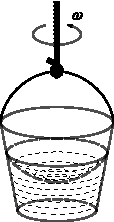
\includegraphics{figure/fig12.11b}}
  \caption{牛顿的水桶实验}
  \label{fig:12.11}
\end{figure}

\vspace{1em}
牛顿的水桶判别法受到反对绝对时空的人的批评。最有
力的批评是马赫给出的。马赫在《发展中的力学》一书中写
道:
\begin{quoting}
  “如果我们说一个物体$ K $只能由于另一物体$ K' $的作用
  而改变它的方向和速度,那么,当我们用以判断物体K的运
  动的其他物体$ A,B,C,\dots $都不存在的时候,我们就根本得
  不到这样的认识,因此,我们实际上只认识到物体同$ A,B,
    C $的一种关系。如果我们现在突然想忽略$ A,B,C,\dots $而
  要谈物体K在绝对空间中的行为,那么我们就要犯双重错误。
  % 366.jpg
  首先,在$ A,B,C,\dots $不存在的情况下,我们就不能知道
  物体$ K $将怎样行动;其次,我们因此也就没有任何方法可以
  用以判断物体$ K $的行为,并用以验证我们的论断。这样的论
  断因而也就没有任何自然科学的意义。”
\end{quoting}

根据这种观点,马赫认为牛顿的水桶实验并不表明绝对空间
的存在。因为,牛顿的实验谈不上是相对于绝对时空来做的,牛
顿水桶周围的宇宙空间里存在着许许多多的物体,原则上说,只
有把这些物体全部拿走,才有可能谈得上是牛顿的绝对空间。这
样,水面的形式,并不反映水桶是否相对于绝对空间有转动,而
是反映水桶相对于地球和其他天体是否有转动。水面变凹,并不是
由于绝对转动所引起的,而是由于宇宙间各种物质对相对于它们
转动的水桶的作用结果。无论是水桶相对于宇宙间物质进行转动,
或者是宇宙间物质相对于水桶在转动,二者结果是一样的,水面
都会同样地变凹。因此,水面变凹仅仅能证明水桶与宇宙间其他
物质($ A,B,C,\dots $)间有相对转动而不能证明绝对空间的存在。

我们可以再利用下面的例子简单地表述牛顿和马赫两种观念
的差别。夜间,我们站在星斗之下,我们看到满天的星是静止
的。这时,我们的两臂自然地下垂。当我们突然转动身体时,我
们看到两件事同时发生了,一是星星开始旋转,二是我们的两臂
也被甩向外边。牛顿认为这两件事是没有直接关系的,而是由于
存在第三者—绝对空间,相对于绝对空间的转动引起惯性离心
力,是绝对空间的存在决定了两臂被甩开。相反,马赫认为不存
在这个想象中的第三者。关键是上述同时看到的两种现象之间有
直接的关系。是转动的星的体系决定了两臂的甩开。马赫主张建
立一种更正确的动力学,它应当能说明转动星体如何作用到手臂
上产生了牛顿体系中的“惯性力”。

总之,在马赫的观念中,所谓惯性力并不是来自时空几何度
量系的“虚拟”力,而同样是宇宙间物体之间的相互作用。水面
% 367.jpg
的变凹,手臂的甩开,是由于旋转着的宇宙天体对于水及手臂作
用的结果。

到此,两种观点有了很大的分歧,但还没有多大实质上的差
别。因为两种观点计算水面变凹的程度是一样的,只是解释不
同。马赫的观点认为,惯性力并不是源于抽象的绝对时空,而是
有物质性的,它是物质间真实的作用力,但究竟是什么样的真实
力却不清楚。将此问题更推进一步的是爱因斯坦。他把问题倒过
来,看到有些真实力在某种意义上很象牛顿意义下虚拟的惯性
力。有这种性质的真实的力就是引力。

由式\eqref{eqn:12.01.03}、\eqref{eqn:12.02.03}、\eqref{eqn:12.02.06}及\eqref{eqn:12.02.07}看到,惯性
力的基本特点是与质点的质量成正此。引力$ F = m \dfrac { G M } { r ^ { 2 } } $也有这种
特点。其他的基本作用力,如电磁力等,则没有这种特点。因此,
在某种意义上就无法区别引力和惯性力。最简单的例子是地球的
重力场。在地球表面附近,质量为$ m $的质点受到的重力是
\begin{equation*}
  \vec{F} = m \vec{g}
\end{equation*}
\begin{wrapfigure}[8]{r}{13.5em}
  \vspace{-2em}
  \centering
  \subfigure[\label{fig:12.12a}]{
\includegraphics{figure/fig12.12a}}
  \subfigure[\label{fig:12.12b}]{
\includegraphics{figure/fig12.12b}}
  \caption{}
  \label{fig:12.12}
\end{wrapfigure}
坐在完全封闭的电梯里的观
察者,看到物体以加速度$ \vec{g} $
向下落,如图\ref{fig:12.12a}所示。
他认为是物体在地球重力作
用下自由下落,电梯里另外
一个观察者完全可以认为根
本没有地球,是地球以加速
度$-\vec{g}$在运动,如图\ref{fig:12.12b}
所示。因此,与在伽利略大船里无法判断绝对速度一样,电梯里
的观察者也无法判断有没有地球存在;或者说无法判断引力的大
小是多少;或者说无法判断绝对加速度是多少。这就是说,在电
梯内所有实验无法判断加速度是由引力引起的,还是由惯性力引
% 368.jpg
起的。因此,在这个意义下,引力的作用和惯性力的作用不可区
分。这种不可区分性说明在某种意义下两者是一回事。这就是现
代的观点。

在牛顿的引力理论中,就已发现引力的几何性,但无法说明
其原因。爱因斯坦把伽利略大船的“绝对速度不可测”发展到
“绝对加速度不可测”。正是由于这一点,引力相当于某种惯性
力,或者说,引力具有惯性力的性质。而惯性力在牛顿意义下是
一种完全由时空决定的力,即具有几何性。所以,引力具有几何
性。爱因斯坦从这种观点出发,导出新的引力理论——广义相对
论。它预言了牛顿引力理论中所没有的一些新现象。事实证明,
爱因斯坦的引力理论是正确的,而牛顿的引力理论则不正确。

{马\ziju{-0.005pt}赫由“物理概念要求可测”的基本观点出发,对牛顿的绝
对时空基本参考系进行批评,进而发展为爱因斯坦的广义相对
论。在物理学上,这是物理概念要求有观测基础的一个出色例证。}

当时,马赫批评牛顿的绝对时空,曾被很多人反对。因为人
的日常生活的直观感觉的确认为时空是绝对的。牛顿写的对绝对
时空的描述是人的粗浅感觉的总结。但这种总结是不正确的。
我们必须用严格的物理方法来审查它,即这样一种绝对时空到底
能不能被测量,直观的感觉有时是错误的,很多人反对马赫的批
评,也是自然的事情。但历史证明马赫的这个批评是正确的。
